\documentclass{beamer}
\usetheme{metropolis}
\usepackage{graphicx}
\usepackage{amsmath}
\usepackage{tcolorbox}
\title{College Writing Seminar (INTD100): Week 3 Notes}
\author{Jordan Hanson}
\institute{Whittier College Department of Physics and Astronomy}

\begin{document}
\maketitle

\section{Summary}

\begin{frame}{Summary}
\textbf{Week 3}: \textit{Technical description I:} In Week 3, we will focus on removing ambiguity from descriptions of a wide variety of situations including (a) scenes or settings, (b) drawings or diagrams, and (c) locations on the map or in a space.
\begin{itemize}
\item Exercises: Working in pairs, describe the location of an object in a photograph without revealing what it is to the other, then writing that down
\item Exercises: Working in pairs, describe a technical diagram with the goal of developing instructions for assembly
\item Homework: write an unambiguous set of instructions for executing a task like the performance of a scientific experiment, procedure, or calculation
\item Exploration topic: COVID-19 and pandemics
\end{itemize}
\end{frame}

\section{Introduction to Technical Description}

\begin{frame}{Introduction}
\textit{\alert{Many people think they can describe something.}} - Have you ever been in a situation in which you were \textit{sure} someone understood you, only to find out they had the wrong idea?  What is required of good technical description?
\begin{enumerate}
\item \textbf{Specific details}
\begin{itemize}
\item Spatial: location in 2D/3D space, geographic
\item Temporal: order, past or future
\item Observable: shape, color, structure, orientation
\end{itemize}
\item \textbf{Objective details}
\begin{itemize}
\item Which way is up? Discussions of physical perspective
\item Dispassionate description
\item Removal of ambiguous words
\end{itemize}
\end{enumerate}
\textbf{Why is this necessary to study and practice?} Science, which relies on the scientific method, is impossible without \textit{repeatability}.
\end{frame}

\begin{frame}{Introduction}
Writing activity: in pairs (partner 1 and partner 2), in breakout rooms:
\begin{enumerate}
\item An image will be displayed on the next slide.  Partner 1 will choose an object in the image.
\item Partner 1: describe the object to Partner 2 such that they can identify it.
\item Partner 2: tell Partner 1 your guess.  If you get it right, give Partner 1 a point.
\item Trade roles: Partner 1 becomes Partner 2 and vice versa.
\item Repeat as many times as possible within the time allowed.
\item Submit high score to group chat for bragging rights.
\item \textit{Note: you cannot just say the name of the object and give it away.  Describe it somehow...}
\end{enumerate}
\end{frame}

\begin{frame}{Introduction}
\begin{figure}
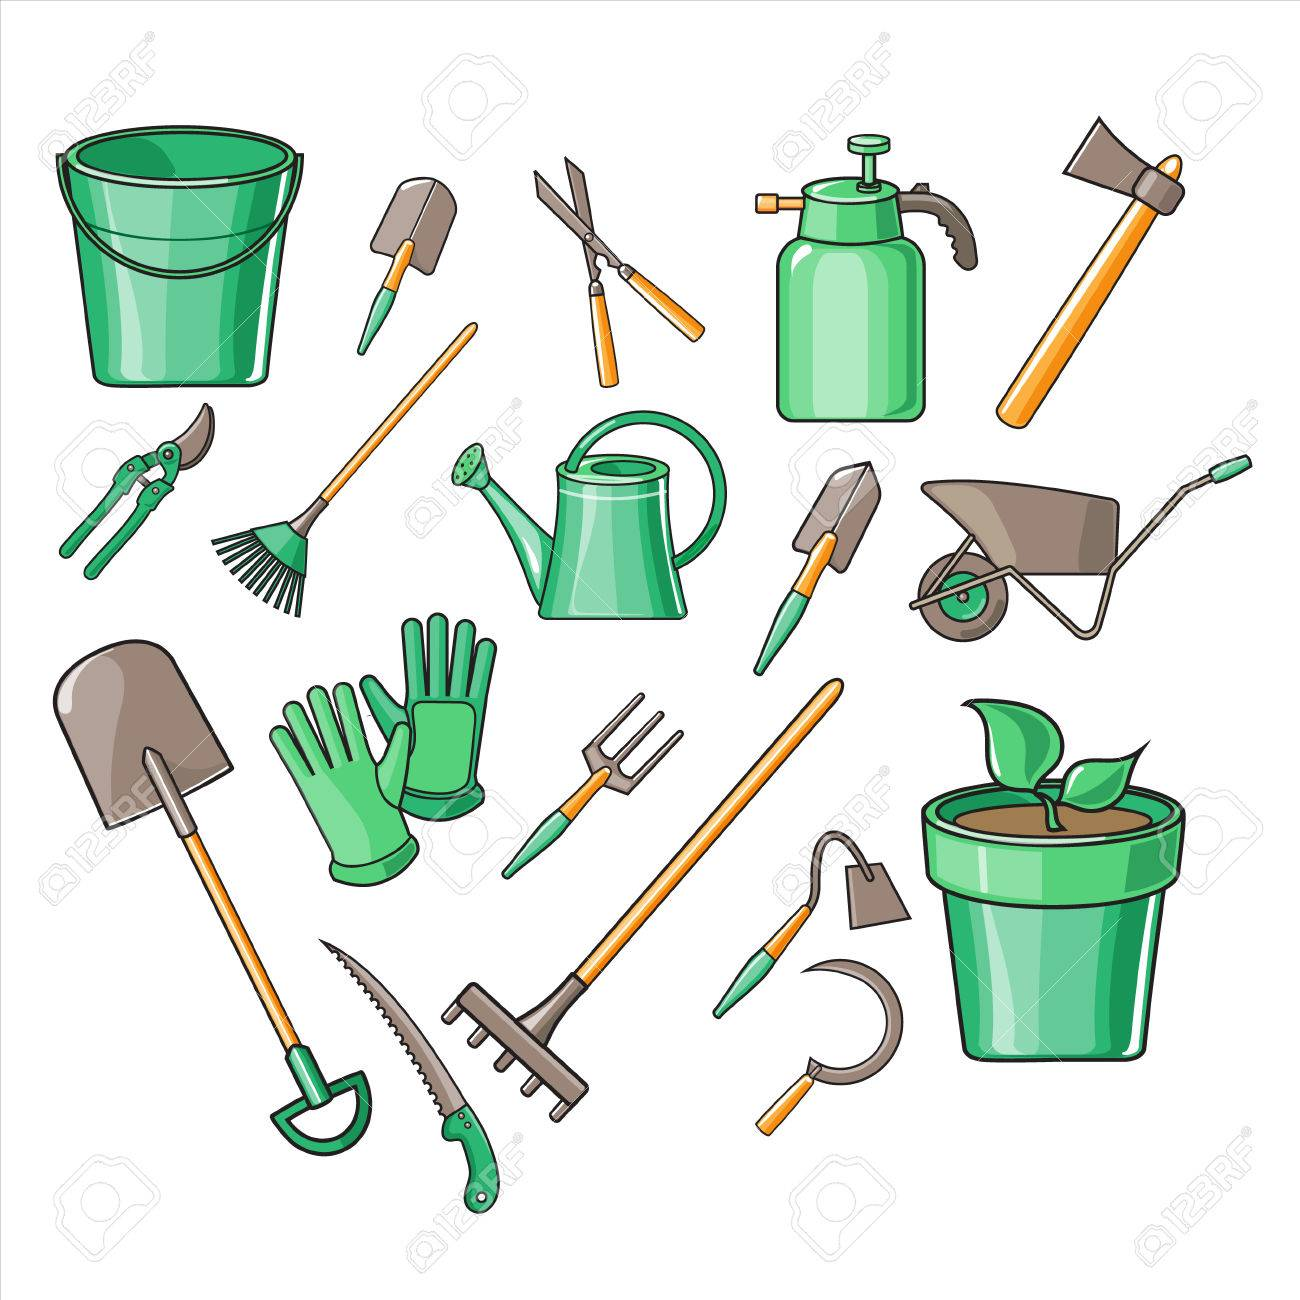
\includegraphics[width=7cm]{figures/garden1.jpg}
\caption{\label{fig:garden1} Round one image.}
\end{figure}
\end{frame}

\begin{frame}{Introduction}
What was your high score?
\begin{figure}
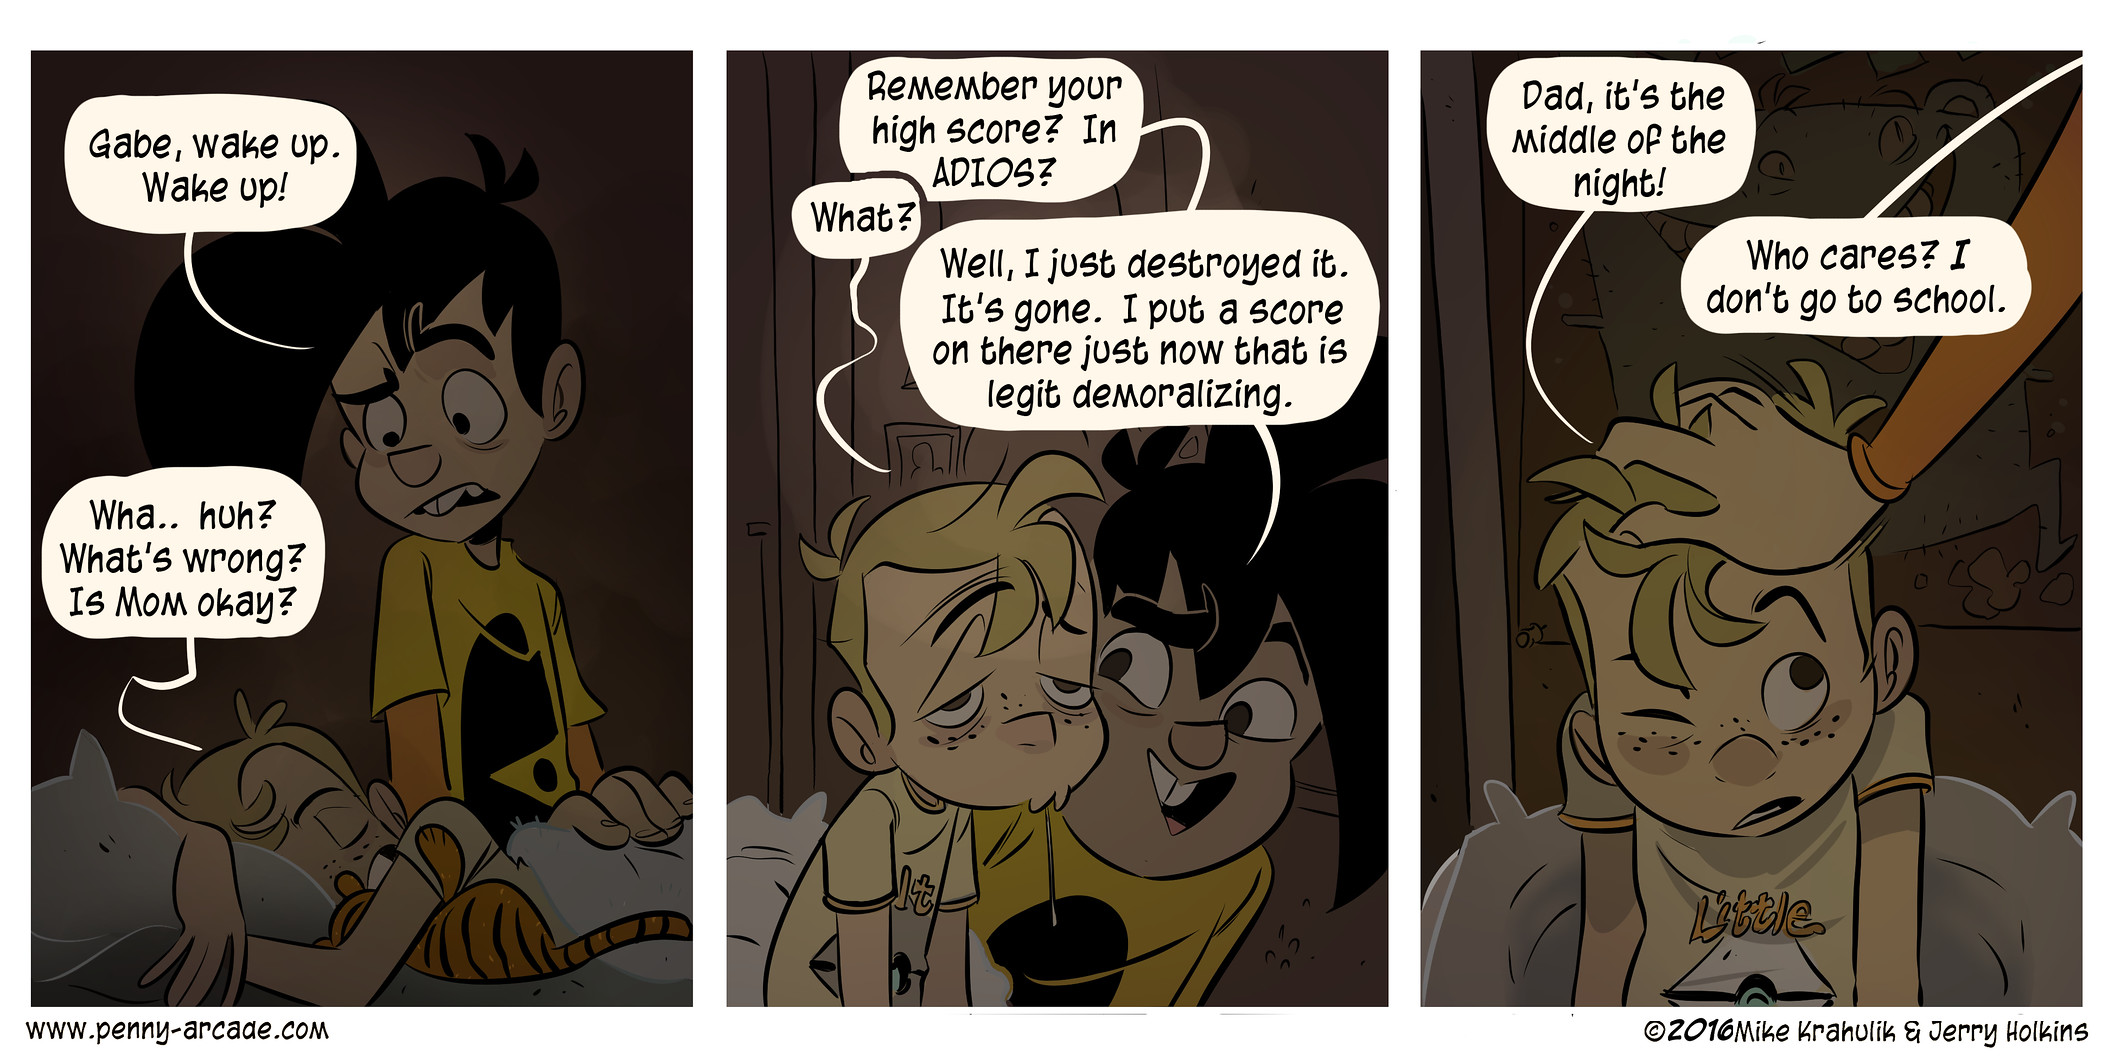
\includegraphics[width=11cm]{figures/funny.jpg}
\caption{\label{fig:funny} Penny Arcade is awesome.}
\end{figure}
\end{frame}

\begin{frame}{Introduction}
\begin{figure}
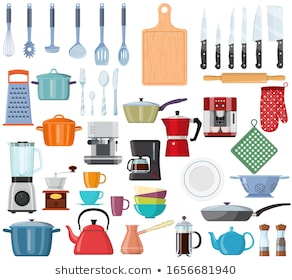
\includegraphics[width=7cm]{figures/kitchen1.jpg}
\caption{\label{fig:kitchen1} Round two image.}
\end{figure}
\end{frame}

\begin{frame}{Introduction}
Notice that there is \textit{more than one way to win.}
\begin{itemize}
\item Describing the shape/color of the object
\item Describing the location of the object
\item Describing the purpose of the object
\item Describing the order or orientation of the object
\item Use unambiguous words.
\end{itemize}
Ready for the last round?  Three, two, one ... go!  First place gets a free Dr. Pepper.
\end{frame}

\begin{frame}{Introduction}
\begin{figure}
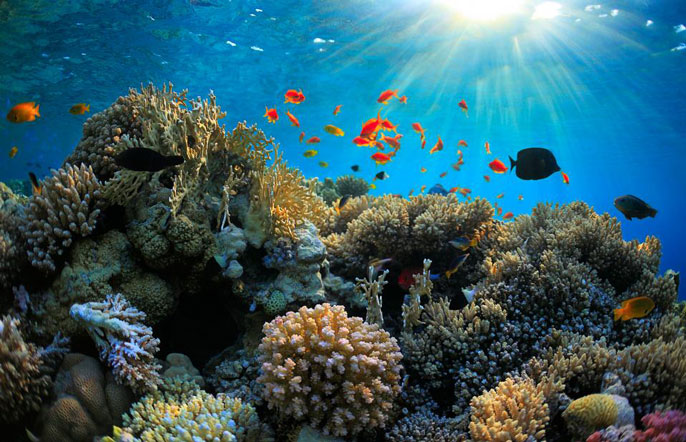
\includegraphics[width=10cm]{figures/coral1.jpg}
\caption{\label{fig:coral1} Round three image.}
\end{figure}
\end{frame}

\begin{frame}
\textbf{Winner winner, chicken dinner.}
\end{frame}

\section{Specific Details: Spatial Detail}

\begin{frame}{Spatial Detail}
In science writing, spatial detail is often critical in understanding experimental results.  \textit{Where specifically} did the expedition take place?  Where specifically on the large protein does the ligand bond? \\ \vspace{0.25cm}
\textbf{Activity:} Look near your laptop/mobile device.  Select an object that is within reach.  Write a description that would allow someone to locate the object by starting from your front door or the entrace to your building (note: obviously we don't have each other's addresses).  Notice how \textit{detailed} you must be.
\end{frame}

\begin{frame}{Spatial Detail: Example}
\textbf{My rosary:} Beginning at my front door, you must enter and take several steps forward into the hallway.  Turn left into the living room and pass the windows on your right side.  In front of you, there is a folding table serving as a desk.  On the left side of the desk as you face it, there is a small collection of personal items behind the stack of notebooks.  The rosary is among these items, and is made from silver metallic beads.
\end{frame}

\begin{frame}{Spatial Detail: Example of parity}
\textbf{Which way is left?} (First time we'll discuss, also in \textit{objective details section}).  What do you mean by left or right?  Up or down? \\
\begin{itemize}
\item From the perspective of the \textit{reader} or the \textit{author}?
\item Is there a more specific way to locate the object?
\begin{itemize}
\item Next to what is the object?
\item Is there a coordinate system defined
\item (For maps) does the object have longitude and latitude (or can you use the compass)?
\end{itemize}
\item Has ``left'' changed since the perspective of the reader has moved in 3D space?
\end{itemize}
\textbf{Professor:} Relate back to the example on prior slide.
\end{frame}

\begin{frame}{Spatial Detail: Example of coordinates}
\begin{figure}[ht]
\centering
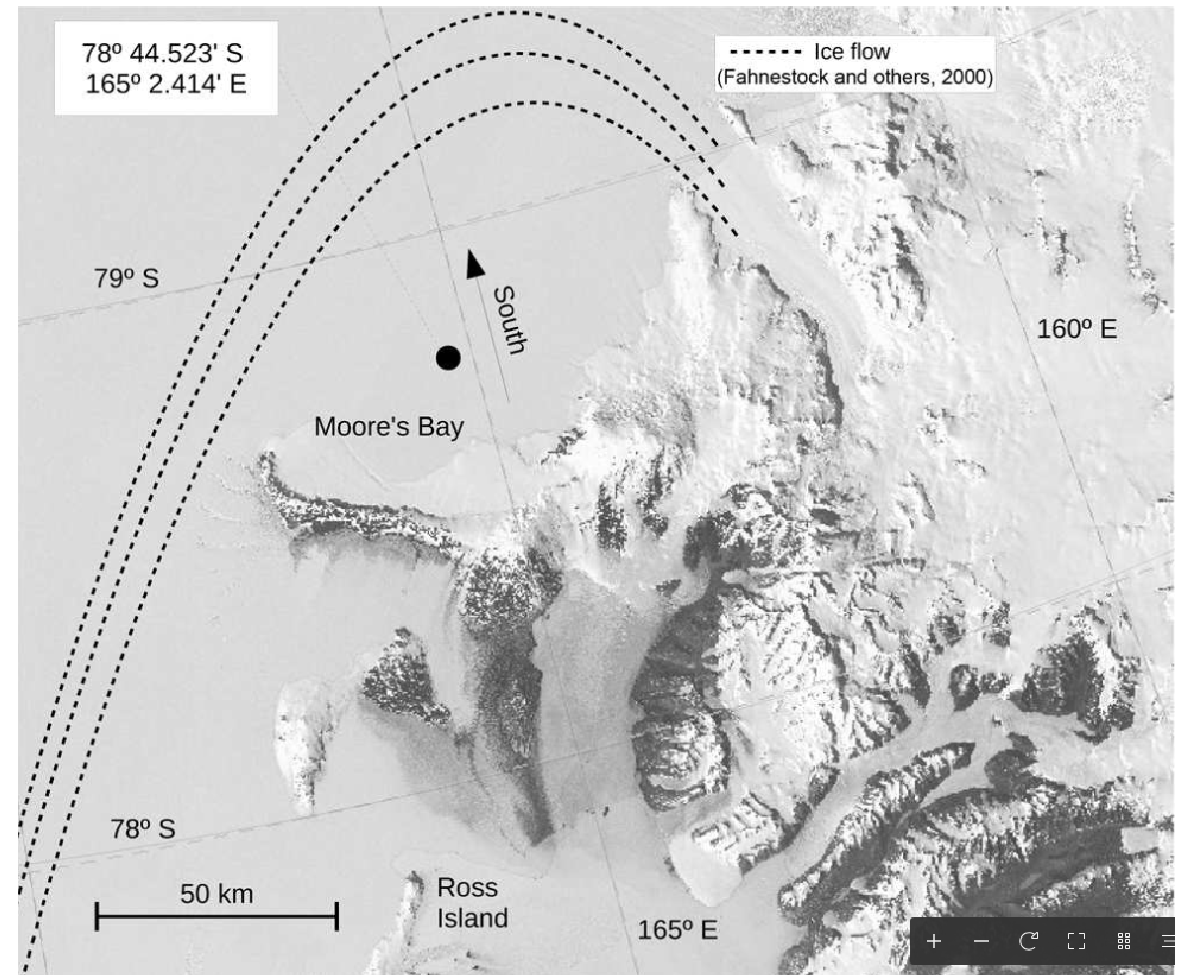
\includegraphics[width=7cm]{figures/NavigationMazePlain.pdf}
\caption{\label{fig:maze1} A map of the McMurdo-Moore's Bay Area.  One of my larger research projects is located here.}
\end{figure}
\end{frame}

\begin{frame}{Spatial Detail: Example of coordinates}
\begin{figure}[ht]
\centering
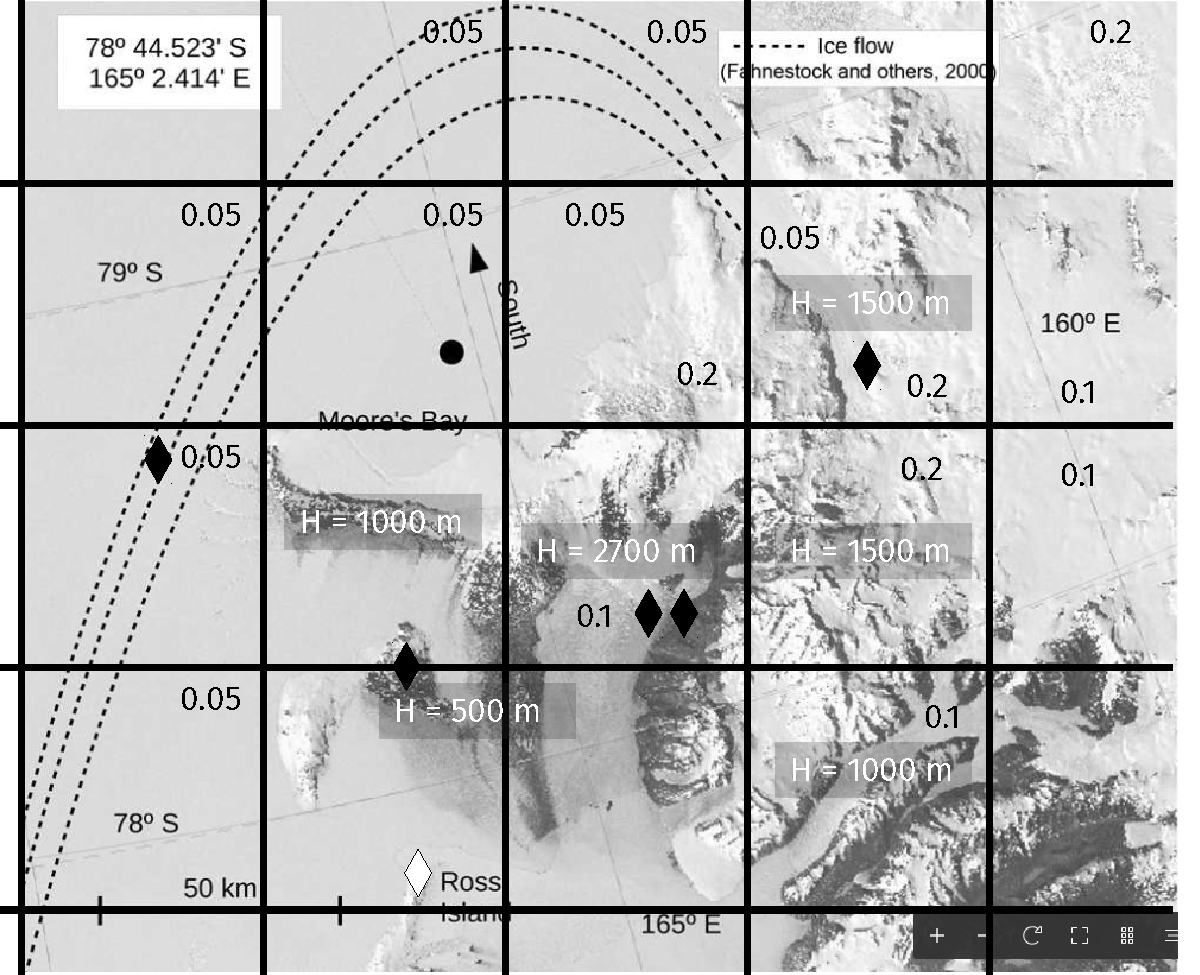
\includegraphics[width=7cm]{figures/NavigationMaze.pdf}
\caption{\label{fig:maze2} A map of the McMurdo-Moore's Bay Area.  Each block is 50 km by 50 km.  The starting point is the white diamond, and the finishing point is the black circle.}
\end{figure}
\end{frame}

\begin{frame}{Spatial Detail: Example of coordinates}
\textbf{Activity:} Describe \textit{exactly} how you would move from McMurdo Station to ARIANNA.
\begin{enumerate}
\item Be precise in your language.
\item Use exact distances, if possible
\item Avoid words like \textit{turn left} in favor of \textit{turn South} or \textit{turn 90 degrees clockwise as you look at the map.}
\item Pay attention to the temporal order of details (more in the next section).
\end{enumerate}
\end{frame}

\section{Specific Details: Temporal Details}

\begin{frame}{Temporal Detail: Example of a Recipe}
\small
\textbf{How do you make beans?} \textit{Como se hacen los frijoles?} \\ \vspace{0.25cm}
\alert{Write the recipe for one of your favorite dishes, from memory}.  Here is an example of mine: \\ \vspace{0.25cm}
First, put two cups of dried pinto or perueno beans in a sieve, and wash them in cold water.  Second, place the washed beans in the pot of a crockpot.  Third, dice half of a white onion, and add the onion to the crockpot.  Fourth, mince two to three cloves of garlic (to taste) and add to the crockpot, along with a sprinkle of salt and pepper (to taste).  Add cold water to the crockpot until the level of water reaches the second knuckle of fingers dipped vertically into the pot.  Close the lid and slow cook for 4-6 hours.  Once complete, heat one to two tablespoons of olive oil in a steel frying pan.  Toast several chiles arbol in the oil until dark red, and then remove them.  Finally, using a ladle, spoon the beans and liquid from the pot into the hot oil and sizzle until cooked into a smooth mixture.  Mash according to preference, and serve hot with fresh tortillas.
\end{frame}

\begin{frame}{Temporal Detail: Example of a Recipe}
\begin{itemize}
\item What if I had switched the order: heat the oil then discussed the crockpot.  That would mean the hot oil was just sitting there for several hours, oops.
\item What if I had added the water to the crockpot \textit{before} adding the beans, onion and garlic to the pot?  What would happen to the measurement of water?
\item Now let's apply this to science writing...
\end{itemize}
\end{frame}

\begin{frame}{Temporal Detail: Experimental Design}
\textbf{Kinesiological measurement.} Sometimes we are interested in measuring how much air someone's lungs can intake.  Describe an experimental design that measures the effect of smoking on lung intake.  Imagine you have some patients who have smoked, some patients who have not smoked, and that you can make them do a little exercise.  Imagine also that you have a device that can record the volume of air the patients inhale per breath for some time duration. \\ \vspace{0.5cm}
\alert{Pay attention to the temporal ordering of your details.  Would someone be able to repeat the experiment you are describing?}
\end{frame}

\section{Specific Details: Objective Detail}

\begin{frame}{Specific Details: Objective Detail}
\textbf{Objective detail} is another skill under the technical description piece of science writing. \\ \vspace{0.3cm}
\textit{Several exercises for practice:}
\begin{enumerate}
\item Which way is up?  Describing an image that by necessity requires the observer to define directions properly
\item \alert{Dispassionate description}: refine descriptive practice in favor of objective observations rather than emotional characterizations
\item Identification and substitution of ambiguous words
\end{enumerate}
\end{frame}

\begin{frame}{Specific Details: Objective Detail}
Objective details: which way is up?  In a moment, you will be shown a map of the northern hemisphere of the Earth.  Two locations are marked: Oslo, Norway, and Anchorage, Alaska. \\
\begin{enumerate}
\item Using a paragraph, describe a path to sail from Oslo to Anchorage.
\item The solution is called \textit{The Northwest Passage.}  Does this sound familiar?
\item You cannot sail North of Greenland, because you would run into polar sea ice.
\item This exercise, and the solution, comes from my INTD255 course: Safe Return Doubtful: History and Current Status of Modern Science in Antarctica
\end{enumerate}
\end{frame}

\begin{frame}{Specific Details: Objective Detail}
\begin{figure}
\centering
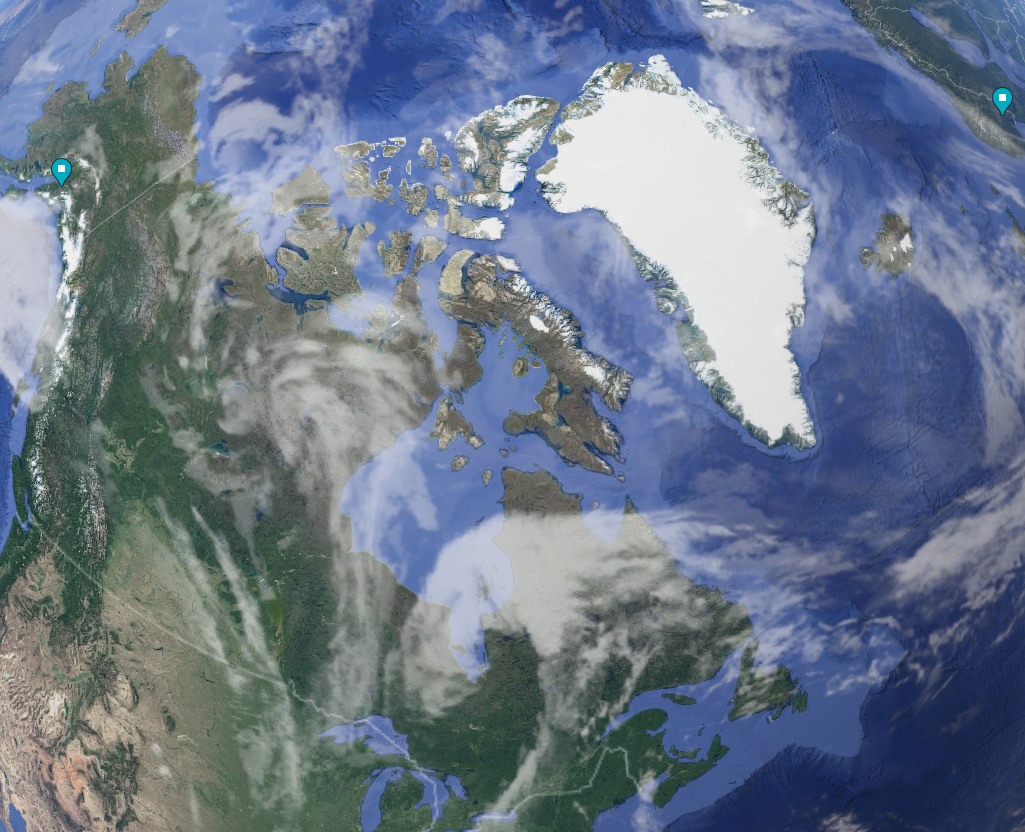
\includegraphics[width=8cm]{figures/path.png}
\caption{\label{fig:globe} (Pin on right): Oslo, Norway.  (Pin on left): Anchorage, Alaska.  North of Greenland is out of bounds.}
\end{figure}
\end{frame}

\begin{frame}{Specific Details: Objective Detail}
\small
\textbf{Example pathway:} Sail West from Oslo with the goal of passing just north of Iceland.  Follow the Eastern coast of Greenland, round the Southern tip of Greenland and head North East.  Following the Western coast of Greenland, aim for the channel between the Eastern Canadian islands and Greenland.  After sailing North an equivalent distance of approximately two-thirds of the length of Greenland, turn West through the first available channel.  Proceed West through the islands, turning North West after passing four main islands.  Re-orient West to the Northern side of Alaska and proceed.  Follow the cost of Alaska until the Bering straight is reached, and finally turn South.  After passing through the Bering strait, locate a gap in the Aleutian islands and follow the coastline East and South until Anchorage is reached.
\end{frame}

\begin{frame}{Specific Details: Objective Detail}
\alert{Dispassionate description}: refine descriptive practice in favor of objective observations rather than emotional characterizations.  In a moment, you will be shown pictures that have cultural implications.  In two to three sentences, describe what you see in these photos. \\
\begin{enumerate}
\item Re-read your sentences.  Are any of the words not \textit{objective?}
\item The goal in scientific or technical writing is not the same as other styles.
\item Compare sentences via discussions in breakout rooms.
\item Technical description is liberating in a way, because another person \textit{should not be able} to disagree with your description or assessment of what's happening in the image.
\end{enumerate}
\end{frame}

\begin{frame}{Specific Details: Objective Detail}
\begin{figure}
\centering
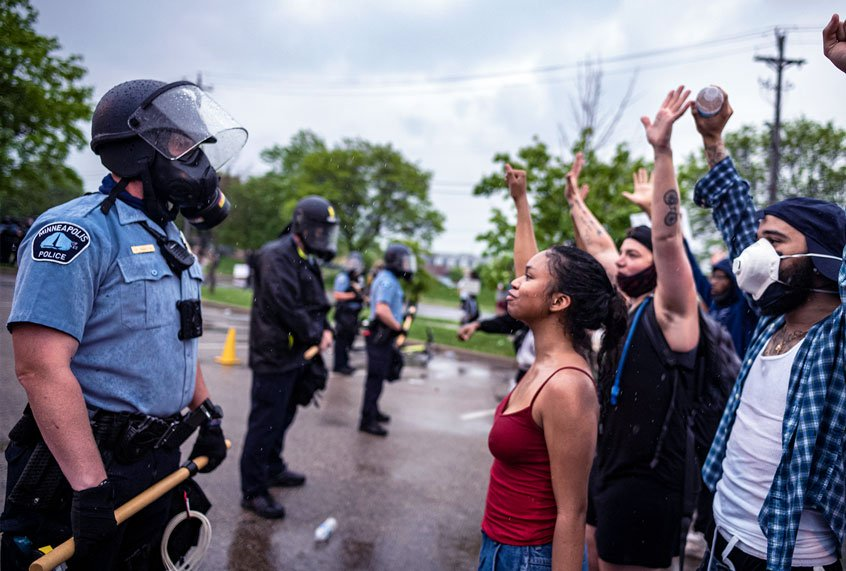
\includegraphics[width=8cm]{figures/passion1.jpg}
\caption{\label{fig:obj1} What do you see?  Describe the scene in two to three sentences.}
\end{figure}
\end{frame}

\begin{frame}{Specific Details: Objective Detail}
\begin{figure}
\centering
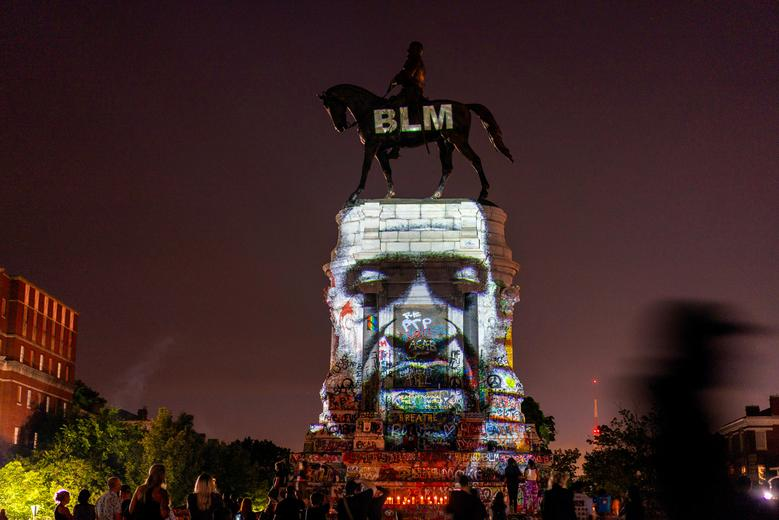
\includegraphics[width=8cm]{figures/statue.jpeg}
\caption{\label{fig:obj2} What do you see?  Describe the scene in two to three sentences.}
\end{figure}
\end{frame}

\begin{frame}{Specific Details: Objective Detail}
\begin{figure}
\centering
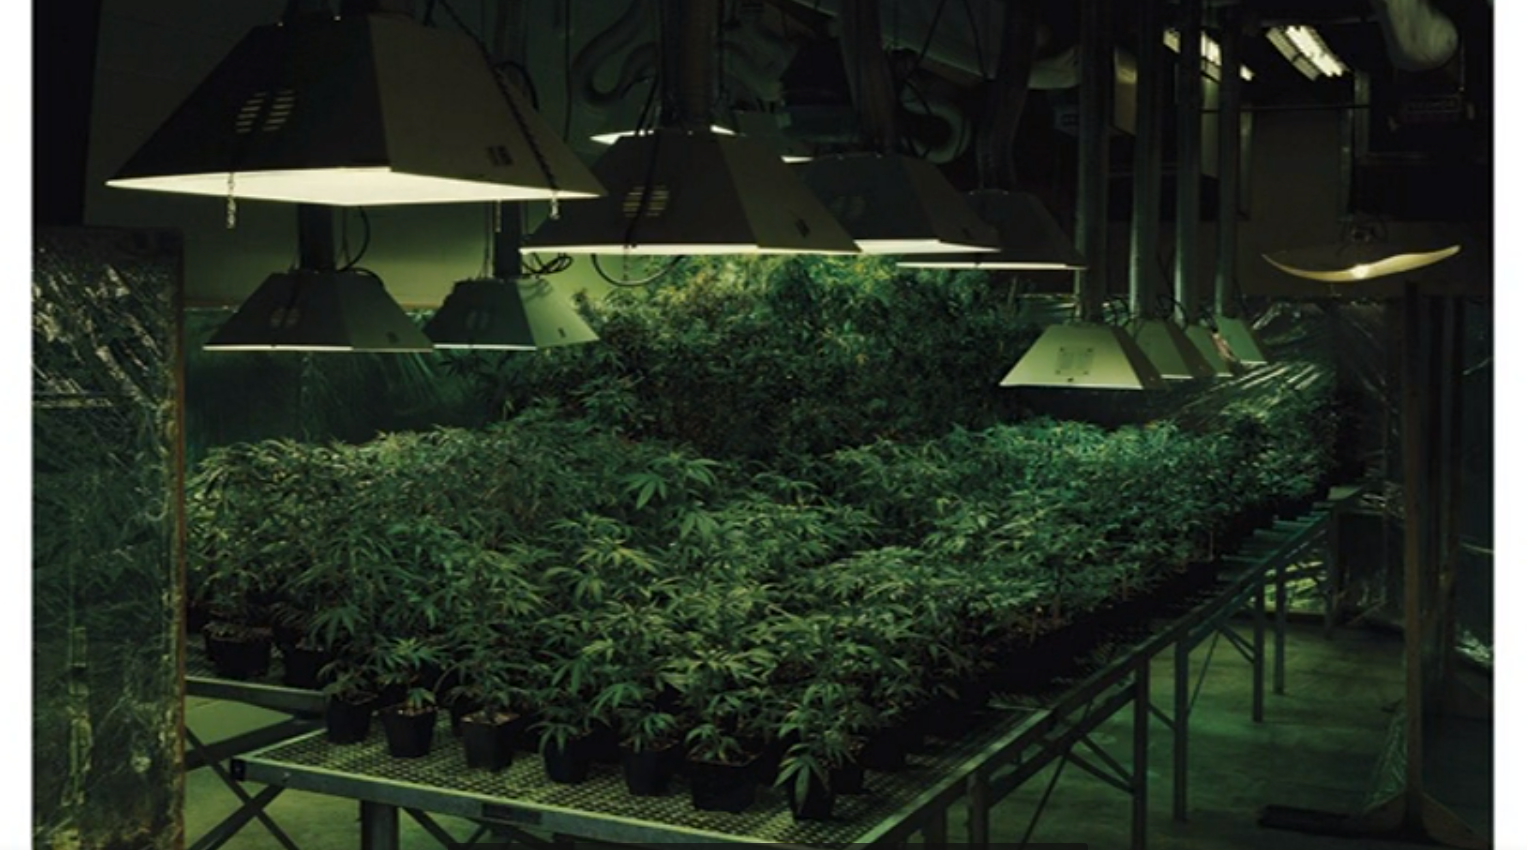
\includegraphics[width=8cm]{figures/weed.png}
\caption{\label{fig:obj3} What do you see?  Describe the scene in two to three sentences.}
\end{figure}
\end{frame}

\section{Specific Details: Removal of Ambiguous Words}

\begin{frame}{Specific Details: Removal of Ambiguous Words}
...
\end{frame}

\section{Conclusion}

\begin{frame}{Conclusion}
\textbf{Week 3}: \textit{Technical description I:} In Week 3, we will focus on removing ambiguity from descriptions of a wide variety of situations including (a) scenes or settings, (b) drawings or diagrams, and (c) locations on the map or in a space.
\begin{itemize}
\item Exercises: Working in pairs, describe the location of an object in a photograph without revealing what it is to the other, then writing that down
\item Exercises: Working in pairs, describe a technical diagram with the goal of developing instructions for assembly
\item Homework: write an unambiguous set of instructions for executing a task like the performance of a scientific experiment, procedure, or calculation
\item Exploration topic: COVID-19 and pandemics
\end{itemize}
\end{frame}

\bibliographystyle{plain}
\section{Bibliography}

\bibliography{bibfile}

\end{document}
